%这是LaTeX源文件
%编译要求:
%编译命令: xelatex -shell-escape rep.tex
%其他要求: 需要安装字体Bitstream Vera Sans Mono;需要安装pygments;需要文档类'cumtbrep';需要实验中用到的代码文件

\documentclass{cumtbrep}

\usepackage{float}
\usepackage{graphicx}
\usepackage{amsmath}
%hyper ref
\usepackage{hyperref}
\hypersetup{colorlinks,bookmarks=false,pdfauthor=王凌峰,pdftitle=报告6}
%font spec
\usepackage{fontspec}
\newfontfamily\bvsm{Bitstream Vera Sans Mono}[NFSSFamily=bvsmfamily]
%code
\usepackage{listings}
\usepackage{minted}
\setminted{breaklines,breakanywhere,mathescape,tabsize=4,style=default,fontsize=\normalsize,fontfamily=bvsmfamily,linenos}
%codes' line number format
\renewcommand{\theFancyVerbLine}{\sffamily
\textcolor[rgb]{0.5,0.5,0.5}{\scriptsize\oldstylenums{\arabic{FancyVerbLine}}}}
%listing's caption
\usepackage{caption}
\captionsetup{tablename=code}
%code with caption
\newcommand\inputcode[3][c++]{%
	\inputminted{#1}{#2}
	\begin{figure}[H]
		\centering
		\captionsetup{type=table}
		\caption{\texttt{#3}}
	\end{figure}
}
\newcommand\inline[2][c++]{\mintinline{#1}{#2}}

\begin{document}

\makeheader{计算机图形学}{王振武}{计科\numberstyle 19-2}{王凌峰}{\numberstyle 1910630221}

\namesec
\begin{enumerate}
	\setcounter{enumi}{5}
	\item 三维几何变换
\end{enumerate}

\purposesec
\noindent 选一种方法

\contentsec
把一个长方体的$x,y$坐标沿原点缩小为$0.3$倍并沿$z$轴旋转$-45^\circ$。

这个实验中比较有趣的地方在于增加了camera transformation $\mathbf{M}_{\mathit{cam}}$,camera coordinate围绕长方体中心旋转,运行中可以在各个方位观察长方体及三维变换后的长方体的形态。

目录结构:{\ttfamily \lstinputlisting{../trans3d/tree}}

camera transformation在运行中不断变化,因此在 \path{trivial.vert} 中声明camera transformation matrix \inline[glsl]{uniform mat4 M_cam},点的位置向量在orthographic transformation之前先进行camera transformation以得到正确的视角。

另外为了方便,orthographic transformation $\mathbf{M}_{\mathit{orth}}$也变化了,新的camera space为
\[
	\left[- \frac{\mathit{windowWidth} - 1}{2},\frac{\mathit{windowWidth} - 1}{2}\right]\times\left[- \frac{\mathit{windowHeight} - 1}{2},\frac{\mathit{windowHeight} - 1}{2}\right]\times\left[-2000,0\right]
\]

\inputcode[glsl]{../trans3d/trivial.vert}{trivial.vert}

\path{main.cc}中先使用 \inline{gen_M} 得到变换矩阵 \inline{M},设置vertex shader中 \inline[glsl]{M} 为 \inline{M}。在主循环中每次循环调用 \inline{gen_M_cam} 得到新的camera transformation matrix \inline{M_cam},使视角不断变化。

长方体只要8个顶点表示,但OpenGL中没有primitive绘制长方体和矩形,需要绘制多个直线或三角形组成长方体。这个实验选择直线连接各个顶点,顶点对在Element Array Buffer(EBO)中存放。绘制直线时,调用 \inline{glDrawElements}。

为了方便,原始长方体中心在$\vec{o}=(0,0,0)$,占据空间$[-300,300]\times[-250,250]\times[-600,-100]$。camera coordinate frame的原点$\vec{e}$以半径$500$绕$(0,200,0)$垂直于$y$轴旋转,视线始终朝向长方体中心,即$\vec{o}$。旋转中心的$y$坐标不在长方体的$y$中点是为了观察到立体的效果。

canonical coordiante frame记为$\langle\vec{o},(\vec{x},\vec{y},\vec{z})\rangle$,camera coordiante frame记为$\langle\vec{e},(\vec{u},\vec{v},\vec{w})\rangle$。依照惯例,坐标系都是右手系,camera coordiante frame视线方向为$-\vec{w}$。

要将canonical coordiantes用camera coordiantes表示,需要对位置向量左乘canonical-to-basis matrix:
\[
	\mathbf{M}_{\mathit{cam}}=
	\begin{bmatrix}
		\vec{u} & \vec{v} & \vec{w} & \vec{e} \\
		0 & 0 & 0 & 1
	\end{bmatrix}^{-1}=
	\begin{bmatrix}
		x_u & y_u & z_u & 0 \\
		x_v & y_v & z_v & 0 \\
		x_w & y_w & z_w & 0 \\
		0 & 0 & 0 & 1
	\end{bmatrix}
	\begin{bmatrix}
		1 & 0 & 0 & -x_e \\
		0 & 1 & 0 & -y_e \\
		0 & 0 & 1 & -z_e \\
		0 & 0 & 0 & 1
	\end{bmatrix}
\]

视点$\vec e = (0,200,0)$。确定view-up vector $\vec t$后,$(\vec u,\vec v,\vec w)$可以由观察方向$\vec g$和$\vec t$构造:
\begin{align*}
	\vec w &= - \frac{\vec g}{\|\vec g\|}, \\
	\vec u &= \frac{\vec t \times \vec w}{\|\vec t \times \vec w\|}, \\
	\vec v &= \vec w \times \vec u.
\end{align*}

三维几何变换矩阵$\mathbf{M}$是简单的矩阵,和二维几何变换实验中的矩阵相同。在三维中的效果是$x,y$坐标沿长方体中心缩小为$0.3$倍,再沿$z$轴旋转$-45^\circ$。

这些都在 \path{main.cc} 中:
\inputcode{../trans3d/main.cc}{main.cc}

\analysesec
\begin{figure}[H]
	\centering
	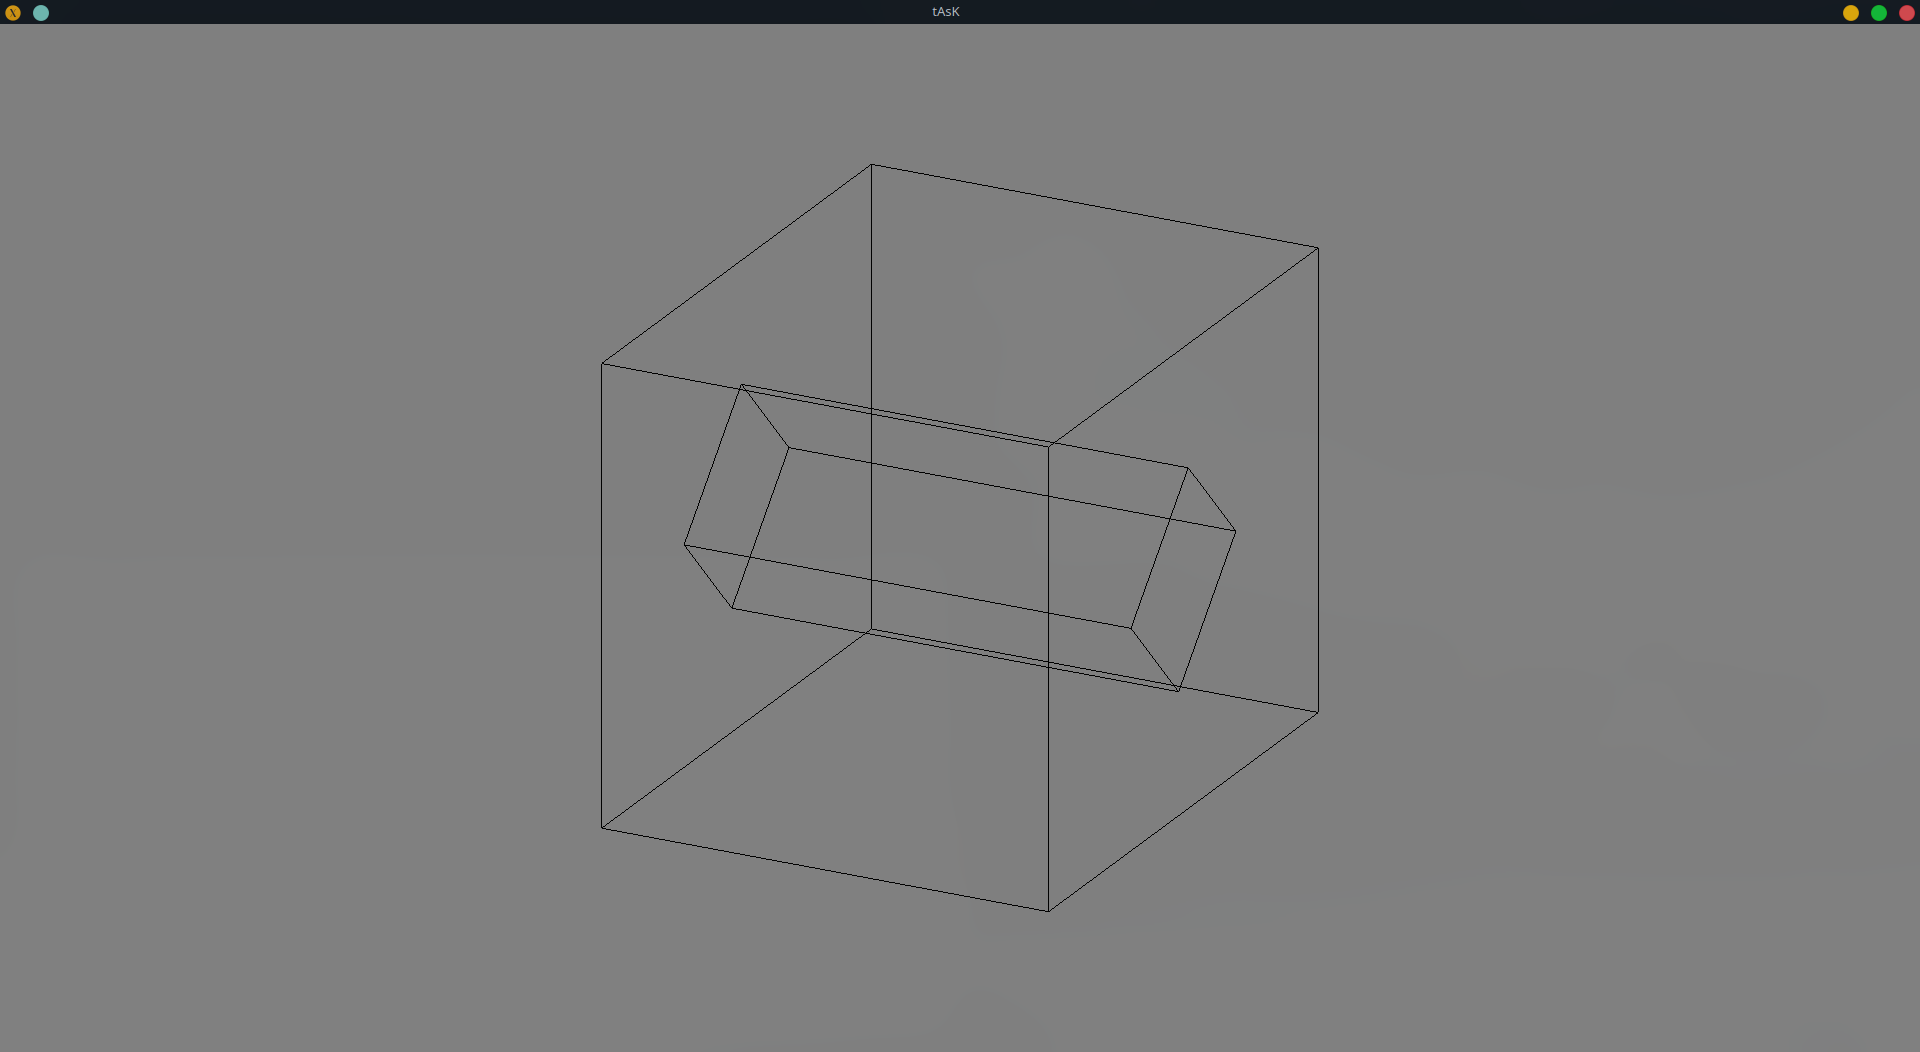
\includegraphics[scale=0.25]{../trans3d/1.png}
	\caption{其中一个视角}
\end{figure}
\begin{figure}[H]
	\centering
	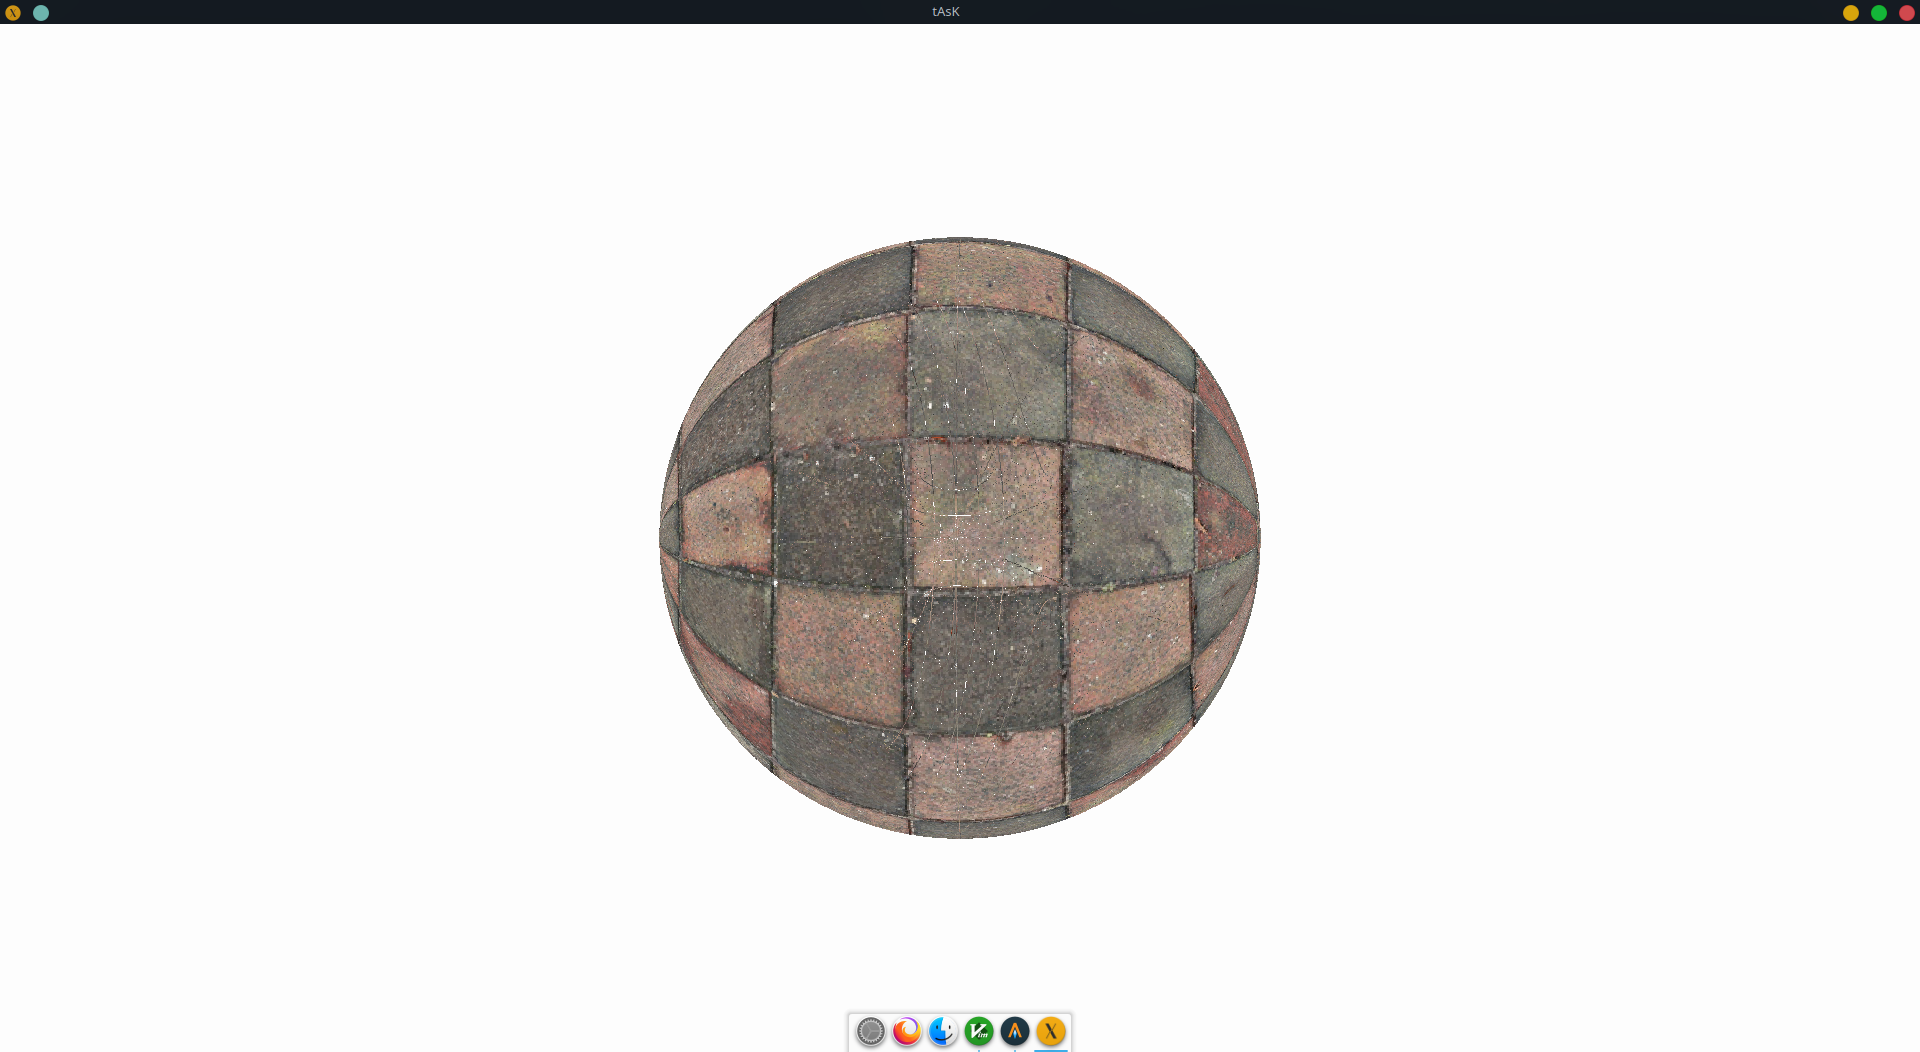
\includegraphics[scale=0.25]{../trans3d/2.png}
	\caption{另一个视角}
\end{figure}

\maketail

\end{document}
